\documentclass[paper=letter, fontsize=11pt]{scrartcl}

\usepackage[T1]{fontenc} % Use 8-bit encoding that has 256 glyphs
\usepackage{fourier} % Use the Adobe Utopia font for the document - comment this line to return to the LaTeX default
\usepackage[english]{babel} % English language/hyphenation
\usepackage{amsmath,amsfonts,amsthm} % Math packages
\usepackage{graphicx}
\graphicspath{{Waveform/}}
\usepackage{lipsum} % Used for inserting dummy 'Lorem ipsum' text into the template
\usepackage{hyperref}

\usepackage{sectsty} % Allows customizing section commands
\allsectionsfont{\centering \normalfont\scshape} % Make all sections centered, the default font and small caps

\usepackage{fancyhdr} % Custom headers and footers
\pagestyle{fancyplain} % Makes all pages in the document conform to the custom headers and footers
\fancyhead{} % No page header - if you want one, create it in the same way as the footers below
\fancyfoot[L]{} % Empty left footer
\fancyfoot[C]{} % Empty center footer
\fancyfoot[R]{\thepage} % Page numbering for right footer
\renewcommand{\headrulewidth}{0pt} % Remove header underlines
\renewcommand{\footrulewidth}{0pt} % Remove footer underlines
\setlength{\headheight}{13.6pt} % Customize the height of the header

\numberwithin{equation}{section} % Number equations within sections (i.e. 1.1, 1.2, 2.1, 2.2 instead of 1, 2, 3, 4)
\numberwithin{figure}{section} % Number figures within sections (i.e. 1.1, 1.2, 2.1, 2.2 instead of 1, 2, 3, 4)
\numberwithin{table}{section} % Number tables within sections (i.e. 1.1, 1.2, 2.1, 2.2 instead of 1, 2, 3, 4)

\setlength\parindent{0pt} % Removes all indentation from paragraphs - comment this line for an assignment with lots of text

%----------------------------------------------------------------------------------------
%	TITLE SECTION
%----------------------------------------------------------------------------------------

\newcommand{\horrule}[1]{\rule{\linewidth}{#1}} % Create horizontal rule command with 1 argument of height

\title{	
\normalfont \normalsize 
\textsc{University of California Irvine} \\  % Your university, school and/or department name(s)
\textsc{Course: Introduction to Digital Logic Lab (31L) Fall 2015} \\ [25pt]
\horrule{0.5pt} \\[0.4cm] % Thin top horizontal rule
\huge Lab 1 Report - Group 9\\ % The assignment title
\horrule{2pt} \\[0.5cm] % Thick bottom horizontal rule
}

\author{Kelvin Phan \\ 51197373
	\and
	Patrick Skoury \\ 75202200
	\and
	Aaron Liao \\ 90811748
	\and
	Shawn Howen \\ 60029119
	\and
	Andrew Mehta \\ 44592437
}

\date{\large\today} % Today's date

\begin{document}

\maketitle % Print the title

%----------------------------------------------------------------------------------------
%	PROBLEM 1
%----------------------------------------------------------------------------------------

\section{Creating the ALU}

%------------------------------------------------

\subsection{Errors Encountered}

\subsubsection{Compilation \\[20pt]} 

\begin{verbatim}
vcom -64 -f rtl.cfg
-- Loading package STANDARD
-- Loading package TEXTIO
-- Loading package std_logic_1164
-- Compiling entity ALU_1bit
-- Compiling architecture Structural of ALU_1bit
** Error: ALU_1bit.vhd(19): near ":": (vcom-1576) expecting IDENTIFIER.
End time: 14:27:55 on Oct 17,2015, Elapsed time: 0:00:00
Errors: 1, Warnings: 0
\end{verbatim}

Resolution: To ensure a successful compilation, it was necessary to remove extra separators ',' in addition to ensuring that all signals were declared with both an identifer and proper type. 

\begin{verbatim}
vcom -64 -f rtl.cfg
-- Loading package STANDARD
-- Loading package TEXTIO
-- Loading package std_logic_1164
-- Loading package NUMERIC_STD
-- Compiling entity addsub
-- Compiling architecture lab1 of addsub
-- Compiling entity sub_borrow
-- Compiling architecture DataFlow of sub_borrow
** Error: sub_borrow.vhd(18): near "OR": (vcom-1576) expecting ';'.
** Error: sub_borrow.vhd(19): VHDL Compiler exiting
End time: 14:55:33 on Oct 17,2015, Elapsed time: 0:00:01
Errors: 2, Warnings: 0
\end{verbatim}

Resolution: When using logic "OR", an error was encountered if other signals/inputs e.g. 'NOT A AND B' were not properly grouped using partentheses () resulting in an error involving resolving logic operators as types or infix expressions.
Successful compilation was achieved when any signals in the form "... + ... + ...", wherein "..." represents a group of inputs and "+" represents "OR", had  parentheses around "...".\\[20pt] 

\subsubsection{Optimization}
\begin{verbatim}
vopt ALU_1bit_tb "+acc=mpr" -o ALUB_1bit_tb_opt

Top level modules:
ALU_1bit_tb

Analyzing design...
-- Loading module ALU_1bit_tb
-- Loading package STANDARD
-- Loading package TEXTIO
-- Loading package std_logic_1164
-- Loading entity ALU_1bit
-- Loading architecture Structural of ALU_1bit
-- Loading package NUMERIC_STD
-- Loading entity addsub
-- Loading entity sub_borrow
-- Loading entity mux81
-- Loading entity mux21
** Error (suppressible): ALU_1bit.vhd(43): (vopt-1270) Bad default binding for 
component instance "addop: addsub".
(Component port "r" is not on the entity.)
** Warning: ALU_1bit.vhd(43): (vopt-3473) Component instance "/ALU_1bit_tb/L1/
addop : addsub" is not bound.
** Error (suppressible): ALU_1bit.vhd(44): (vopt-1270) Bad default binding for 
component instance "subopborrow: sub_borrow".
(Component port "d" is not on the entity.)
** Warning: ALU_1bit.vhd(44): (vopt-3473) Component instance "/ALU_1bit_tb/L1/
subopborrow : sub_borrow" is not bound.
** Error (suppressible): ALU_1bit.vhd(46): (vopt-1270) Bad default binding for 
component instance "subop: addsub".
(Component port "r" is not on the entity.)
** Warning: ALU_1bit.vhd(46): (vopt-3473) Component instance "/ALU_1bit_tb/L1/
subop : addsub" is not bound.
** Error (suppressible): ALU_1bit.vhd(47): (vopt-1270) Bad default binding for 
component instance "increment: addsub".
(Component port "r" is not on the entity.)
** Warning: ALU_1bit.vhd(47): (vopt-3473) Component instance "/ALU_1bit_tb/L1/
increment : addsub" is not bound.
** Error (suppressible): ALU_1bit.vhd(48): (vopt-1270) Bad default binding for 
component instance "decrement: addsub".
(Component port "r" is not on the entity.)
** Warning: ALU_1bit.vhd(48): (vopt-3473) Component instance "/ALU_1bit_tb/L1/
decrement : addsub" is not bound.
** Error (suppressible): ALU_1bit.vhd(49): (vopt-1270) Bad default binding for 
component instance "add_increment: addsub".
(Component port "r" is not on the entity.)
** Warning: ALU_1bit.vhd(49): (vopt-3473) Component instance "/ALU_1bit_tb/L1/
add_increment : addsub" is not bound.
** Error (suppressible): ALU_1bit.vhd(57): (vopt-1270) Bad default binding for 
component instance "outputselectart: mux81".
(Component port "q" is not on the entity.)
** Warning: ALU_1bit.vhd(57): (vopt-3473) Component instance "/ALU_1bit_tb/L1/
outputselectart : mux81" is not bound.
** Error (suppressible): ALU_1bit.vhd(58): (vopt-1270) Bad default binding for 
component instance "outputselectlog: mux81".
(Component port "q" is not on the entity.)
** Warning: ALU_1bit.vhd(58): (vopt-3473) Component instance "/ALU_1bit_tb/L1/
outputselectlog : mux81" is not bound.
** Error (suppressible): ALU_1bit.vhd(60): (vopt-1270) Bad default binding for 
component instance "finaloutputselect: mux21".
(Component port "q" is not on the entity.)
** Warning: ALU_1bit.vhd(60): (vopt-3473) Component instance "/ALU_1bit_tb/L1/
finaloutputselect : mux21" is not bound.
Optimization failed
End time: 15:22:24 on Oct 17,2015, Elapsed time: 0:00:00
Errors: 9, Warnings: 9
\end{verbatim}

Resolution: Failure to properly define components using proper naming conventions in the 1-bit ALU resulted in a "Bad default binding" error during the optimization phase.
To resolve this error, edits were made to the component definitions, ensuring that the input and output identifiers matched those defined in the component's entity.\\[20pt]

\subsubsection{Simulation}
\begin{verbatim}
# ** Warning: (vsim-8683) Uninitialized out port /ALU_1bit_tb/L1/output1 has no 
driver.
# This port will contribute value (U) to the signal network.
# do sim.do
# .
# waveform.wlf
# End time: 15:39:20 on Oct 17,2015, Elapsed time: 0:00:00
# Errors: 0, Warnings: 1
\end{verbatim} 

Resolution: During simulation phase, an error was encountered wherein an output signal was not driven. Signal was then properly assigned/driven to resolve this error. \\[20pt] 

\subsubsection{Logic}
\begin{flushleft}
	1. Delay Problem- Certain operations were not performed because of excessive delay in mux components caused by lack of optimization in data flow design. This prevented the change in "opsel" input from triggering the proper output.\\ 
	To resolve this issue, concurrent "WHEN" and "ELSE" statements were used instead of sum of minterms. "Addsub" component was also optimized through use of "XOR" gates in place of sum of minterms. Decreased delay enabled ALU to run properly.\\[10pt] 

	2. Carry Problem- Arithmetic functions were not able to run or produce outputs because carry values were not being driven properly. This was a result of attempting to drive STD\_LOGIC signal "cin" with multiple sources, which prevented output of proper carry out.\\ 
	To resolve this issue, in "ALU\_32bit.vhd", I set up a base case wherein an initial "cin" is processed and whose value is dependent on the operation being performed. Its initial value is '1' if two's complement subtraction, increment, or add and increment is being performed; otherwise, its value is '0'.
	"cout" was also erroneously driven by multiple sources. Given the use of "GENERATE" to instantiate 1-bit ALUs to form a 32-bit ALU, a "coutbuff" signal defined as a STD\_LOGIC\_VECTOR was used to contain the value of the cout of each ALU in order to carry it to the next. However,
	a base case was used to set up an initial "cin" and "coutbuff" as each "cin" of an ALU following the first 1-bit ALU need to be assigned the value of the previous ALU's "coutbuff".\\[10pt]

	3. Decrement Problem- The decrement function was not producing the correct output due to passing an incorrect value for "B" to each individual ALU. \\In order to resolve this issue, the "addsub" component was used as an adder, setting initial "cin" to '0' and passing '1' for each value of "B" thereby already passing the two's complement of '1' which is '-1'.\\[20pt]
\end{flushleft}

\subsection{Architecture}
\subsubsection{Design for 32-bit ALU}
\begin{flushleft}
	Our design for the 32-bit ALU consisted of instantiating the 1-bit ALU, using a GENERATE statement. The first 1-bit ALU was defined outside of the GENERATE statement in order to separate the carry-in for the 32-bit ALU from the other 31 carry-ins that connect to each 1-bit ALU. A 32-bit vector called "Coutbuff" was defined and set to the carry-out of the 1-bit ALU. Within the GENERATE statement, the carry-in was set to "Coutbuff(i-1)" which allows the carry-out of the previous 1-bit ALU to become the new carry-in. The GENERATE statement was used to copy the 1-bit ALU component 31 times.  	
\end{flushleft}

\subsubsection{Design for 1-bit ALU}
\begin{flushleft}
	The first step within the Architecture of the 1-bit ALU was to define the components we would be instantiating. This included: an 8 to 1 multiplexer, a 2 to 1 multiplexer, and an adder/subtracter, . After defining our signals, a WHEN statement was used to define our signal "optype." This signal was set to '0' or '1' depending on the function and set as an input for the Adder/Subtracter component. The next step was to define all 12 functions that our ALU would perform. The Adder/Subtracter component was instantiated for the Arithmetic operations. The Logic operations did not require any separate components, only simple logic gates. Two 8 to 1 multiplexers were instantiated to differentiate between the seven Arithmetic operations and five Logic operations. The two outputs were set as inputs in a 2 to 1 multiplexer, which was used to choose between the Arithmetic or Logic operation, depending on the input "mode." The output of the 2 to 1 multiplexer was set as the output of the ALU. The last step was to use a WHEN statement to chose what the carry-out would be, depending on "mode" and "opsel." A schematic created with Visio is included below.      
\end{flushleft}
	\centering
			\includegraphics[scale=0.45]{Diagram}
				\label{fig:Diagram}

\section{Waveform Screenshots}

\subsection{Arithmetic Round 1}

	\centering
			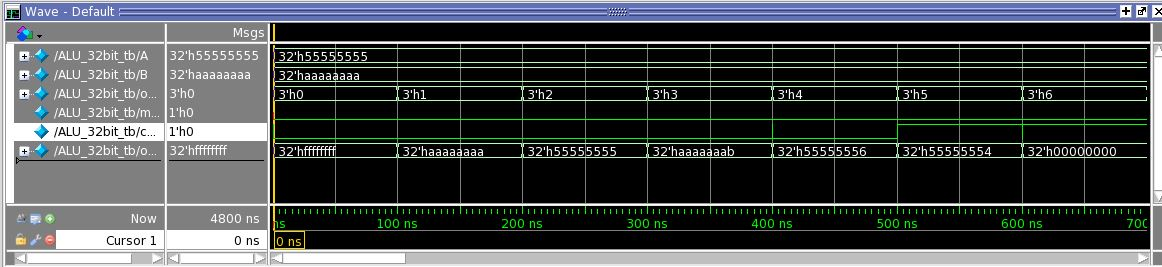
\includegraphics[width=1.0\textwidth]{Art1}
				\label{fig:Art1}
\raggedright A = 32'b01010101010101010101010101010101\\  
B = 32'b10101010101010101010101010101010

\subsection{Arithmetic Round 2}

	\centering
			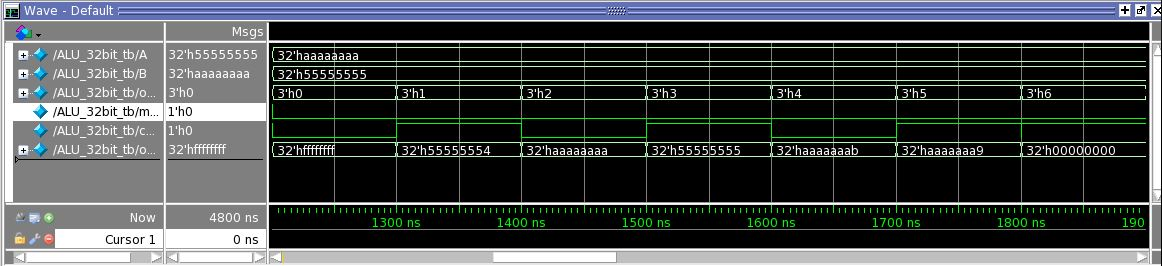
\includegraphics[width=1.0\textwidth]{Art2}
				\label{fig:Art2}
 \raggedright A = 32'b10101010101010101010101010101010\\ 
 B = 32'b01010101010101010101010101010101
 
\subsection{Arithmetic Round 3}

	\centering
			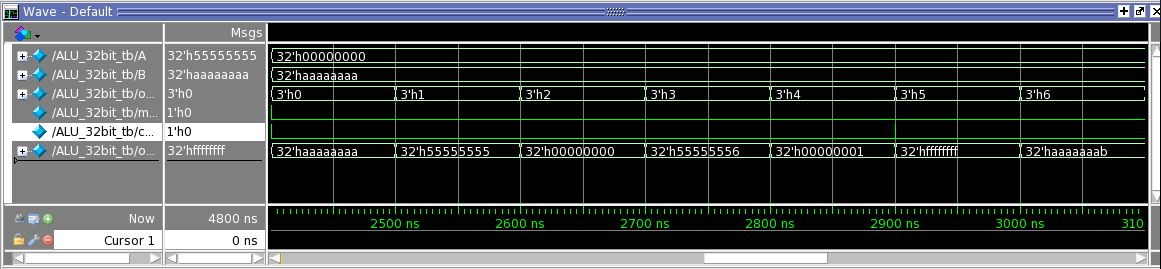
\includegraphics[width=1.0\textwidth]{Art3}
				\label{fig:Art3}
 \raggedright A = 32'b00000000000000000000000000000000\\ 
 B = 32'b10101010101010101010101010101010
 
\subsection{Arithmetic Round 4}

	\centering
			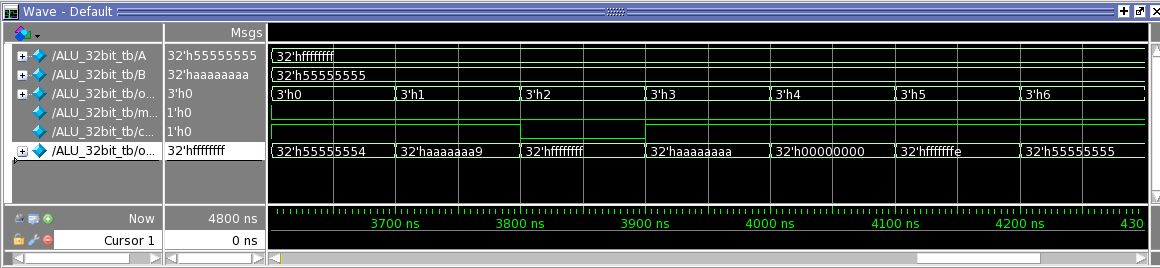
\includegraphics[width=1.0\textwidth]{Art4}
				\label{fig:Art4}
\raggedright A = 32'b11111111111111111111111111111111\\
B = 32'b01010101010101010101010101010101

\subsection{Arithmetic Operations}
\begin{flushleft}
In every round of Arithmetic, the following operations are used according to the input "opsel": \\ [15pt]
1. At 3'h0, Add A + B\\ 
2. At 3'h1, Subtract A - B with a borrowed carry\\
3. At 3'h2, Move A\\
4. At 3'h3, Subtract A - B\\
5. At 3'h4, Increment A by 1\\
6. At 3'h5, Decrement A by 1\\
7. At 3'h6, Add A + B and increment by 1    
\end{flushleft}

\subsection{Logic Round 1}

	\centering
			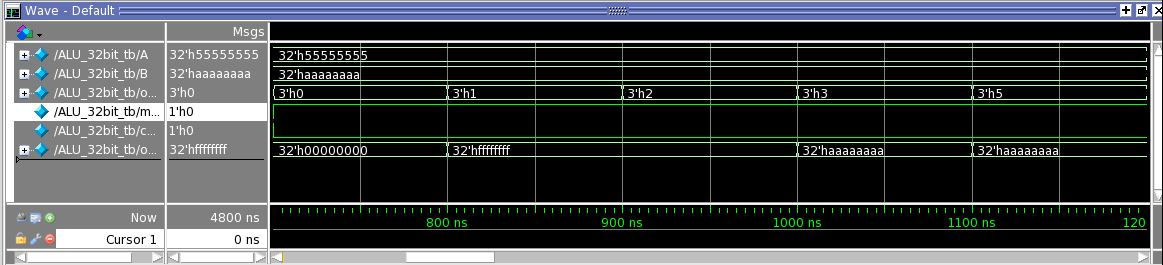
\includegraphics[width=1.0\textwidth]{Log1}
				\label{fig:Log1} \\[-15pt]
\raggedright A = 32'b01010101010101010101010101010101\\  
B = 32'b10101010101010101010101010101010

\subsection{Logic Round 2}

	\centering
			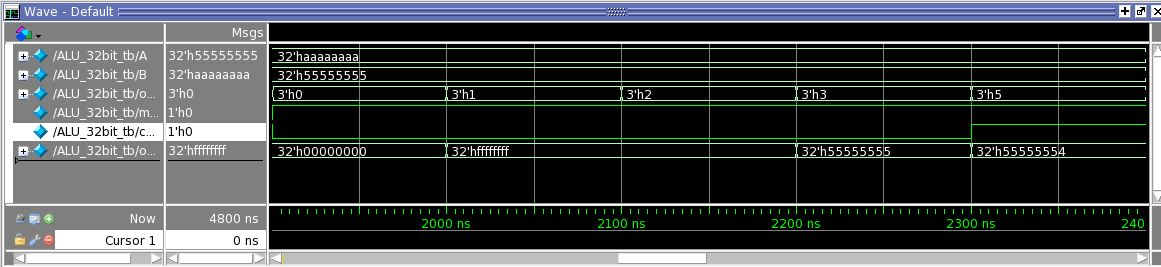
\includegraphics[width=1.0\textwidth]{Log2}
				\label{fig:Log2}
\raggedright A = 32'b10101010101010101010101010101010\\ 
 B = 32'b01010101010101010101010101010101
 
\subsection{Logic Round 3}

	\centering
			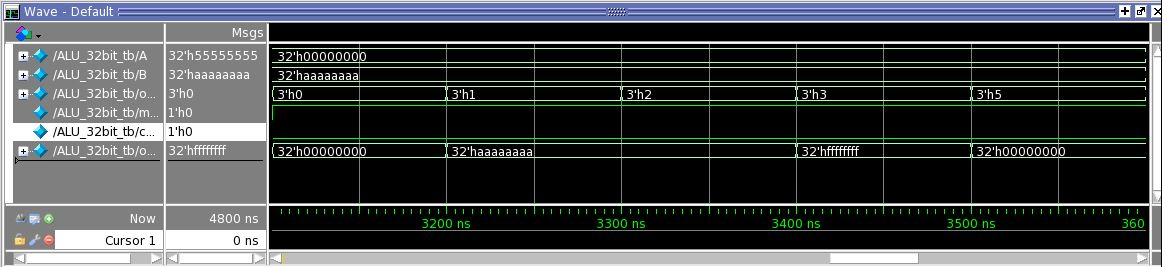
\includegraphics[width=1.0\textwidth]{Log3}
				\label{fig:Log3}
\raggedright A = 32'b00000000000000000000000000000000\\ 
B = 32'b10101010101010101010101010101010

\subsection{Logic Round 4}

	\centering
			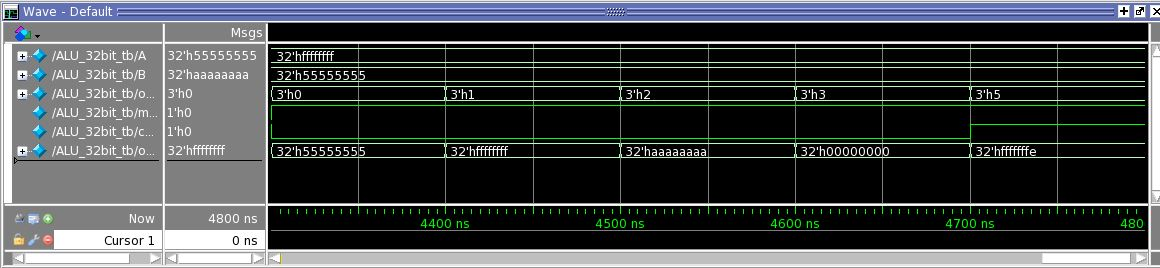
\includegraphics[width=1.0\textwidth]{Log4}
				\label{fig:Log4}
\raggedright A = 32'b11111111111111111111111111111111\\
B = 32'b01010101010101010101010101010101

\subsection{Logic Operations}
\begin{flushleft}
	In every round of Logic, the following operations are used according to the input "opsel": \\ [15pt]
	1. At 3'h0, A AND B\\ 
	2. At 3'h1, A OR B\\
	3. At 3'h2, A XOR B\\
	4. At 3'h3, NOT A\\
	5. At 3'h5, A 32-bit Shift Left (Logic) \\
    
\end{flushleft}
\end{document}
